\documentclass{article}
\usepackage[utf8]{inputenc}
\usepackage[a4paper, portrait, margin=0.6in]{geometry}
\usepackage{graphicx}
\usepackage{subcaption}
\usepackage{amsmath}
\usepackage{geometry}
\usepackage{array}


\title{Software Testing (UE18CS400SB) \\ Unit 1}
\author{Aronya Baksy}
\date{August 2021}

\begin{document}
\maketitle

\section{Introduction}
\begin{itemize}
    
    \item \textbf{Testing}: A process consisting of all life-cycle activities both static and dynamic concerned with \textbf{planning}, \textbf{preparation} and \textbf{evaluation} of a software product and the related work to determine that it \textbf{satisfies the specific requirements} and it fits the purpose, as well as to \textbf{detect defects}
    
    \item Provides stakeholders with info about quality of the software product under test
    
    \item Software testing ensures quality of software and accelerates software development
    
    \item Testing levels: Unit test, integration test, system test and acceptance test
\end{itemize}

\section{Software Quality}
\begin{itemize}
    \item Quality is conformance to standards or requirements (PMBOK)
    
    \item \textbf{ISO 9000}: totality of features and characteristics of a product/service that bear on its ability to satisfied stated and implied needs
    
    \item \textbf{IEEE definition} of quality: 
    \begin{itemize}
        \item The degree to which a system/component/process meets requirements
        
        \item The degree to which a system/component/process meets user needs or expectations
    \end{itemize}
    
    \item \textbf{Pressman's definition} of quality: Conformance to explicitly stated functional and performance requirements, explicitly documented development standards and implicit characteristics that are expected of all professionally developed software
    
    \item Quality is a process than a product. A continuous process of improvement and use of lessons learnt in the past to enhance processes
    
    \item Software defects are costly (money/reputation/danger to human life)
    
    \item Reasons for software failures:
    \begin{itemize}
        \item Uniqueness of the product
        
        \item High complexity
        
        \item Limited opportunities to detect bugs
        
        \item Software dev environment
        
        \item Teamwork
    \end{itemize}
\end{itemize}

\subsection{Software Quality Factors}
\begin{itemize}
    \item \textbf{Correctness}: With regards to conforming to requirements
    
    \item \textbf{Reliability}
    
    \item\textbf{Efficiency}
    
    \item \textbf{Usability}
    
    \item \textbf{Maintainability}
    
    \item \textbf{Flexibility} with regard to changing requirements and adding functionality 
    
    \item\textbf{Testability}
    
    \item\textbf{Portability} across platforms and environments (cloud or native)
    
    \item\textbf{Interoperability} with other services and products
    
    \item\textbf{Reusability}
\end{itemize}

\subsection{Deming's PDCA Cycle}
\begin{itemize}
    \item \textbf{Plan} improvements to existing practices (establish objectives and processes needed to deliver them)
    
    \item \textbf{Do}: Implementation of the plan and objectives of the previous step
    
    \item \textbf{Check} to see if desired results are achieved (compare with expected outcomes to measure similarity and differences)
    
    \item \textbf{Act}: Implement corrective solutions, process improvement appens in this phase
\end{itemize}

\subsection{Cost of Quality}
\begin{itemize}
    \item Total price of all effort needed to achieve product/service quality (3-5\% of total program cost devoted to cost of quality)
    
    \item The quality cost has 4 main components:
    \begin{itemize}
        \item \textbf{Prevention Cost}
        
        \item \textbf{Appraisal Cost}
        
        \item \textbf{Internal Failure Cost}
        
        \item \textbf{External Failure Cost}
    \end{itemize}
\end{itemize}

\subsection{Project Quality Management}
\begin{itemize}
    \item The processes required to ensure that the project satisfies the needs for which it was undertaken
    
    \item Includes all activities of which the overall management function that determine the quality policy, objectives and responsiblities and implements them using quality planning, assurance, control and improvement within the quality system.
    
    \item PQM addresses both management and end product of the project
\end{itemize}

\subsubsection{PQM Processes}
\begin{itemize}
    \item \textbf{Quality Planning}
    \item \textbf{Quality Assurance}
    \item \textbf{Quality Control}
    \item \textbf{Quality Improvement}
\end{itemize}
\begin{figure}[!h]
    \centering
    \begin{tabular}{|c|c|}
        \hline
        \textbf{Quality Assurance} & \textbf{Quality Control}  \\
        \hline
        Process-oriented & Product-oriented \\
        \hline
        Focus on preventing quality issues & Focus on identifying quality issues in products \\
        \hline
        Performed throughout the cycle & Performed after product is built \\
        \hline
        A staff function & Line function \\
        \hline
        e.g.: Reviews, Audits & e.g.: Software testing at various levels\\
        \hline
    \end{tabular}
\end{figure}

\subsubsection{Quality Control using Fish-Bone Analysis}
\begin{itemize}
    \item A multi-purpose representation used for brainstorming, but is mostly used for cause-effect analysis
    
    \item The fish head represents the effect that is observed
    
    \item The bones on the fish's spine represent the causes of the effect that was observed
    
    \item Used in Agile-based development life cycles like Scrum and Kanban
    
    \item Steps in building a Fish-bone diagram:
    \begin{enumerate}
        \item Agree on the problem statement (\textbf{effect}). This forms the fish head. The problem statement must be clear, specific but not defined in terms of any solutions.
        
        \item Agree on major categories of \textbf{causes}. These are the branches on the fish spine
        
        \item Brainstorm all possible causes of the problem. As each idea is put forth, the facilitator puts it on the appropriate category (branch) of the diagram
        
        \item Ask "why does it happen" and form sub branches from the main branches
        
        \item Generate deeper levels of causes and organize them under relevant categories of causes.
    \end{enumerate}
\end{itemize}

\section{Software Developement Life Cycle}
\begin{itemize}
    \item Generic phases of SDLC: Requirement analysis, planning, design, implementation, testing, deployment and maintenance
    
    \item \textbf{Verification}: Evaluating whether the product of a particular phase satisfies the conditions imposed at the start of that phase
    
    \item \textbf{Validation}: Evaluating a system/component during or at the end of the development process to determine whether it satisfies the specified requirements.
    
    \item Every phase of SDLC is characterized by: entry, task, verification, and exit activities.
    
    \item Attributes of an SDLC model:
    \begin{itemize}
        \item Activities performed the sequence and their deliverables
        
        \item Methods of validation and deliverables
        
        \item Methods of verification for each activity, including communication mechanisms between activities
    \end{itemize}
\end{itemize}

\subsection{Waterfall Model}
\begin{itemize}
    \item Progress through each phase flows from top to bottom, in a cascading manner.
    
    \item \textbf{Strengths}: simple, useful for projects divided into components
    
    \item \textbf{Drawbacks}: Delay in feedback among phases, errors in one phase are not detected till next one
\end{itemize}

\subsection{Prototyping Models}
\begin{itemize}
    \item Early and frequent feedback increases chances of meeting customer requirements, and allows project to adapt to rapid changes easily
    
    \item \textbf{Prototyping}: constant user interaction produces a prototype from which the SRS is derived. Prototype is discarded after this, and then the development proceeds once client accepts the SRS
\end{itemize}

\subsection{Iterative Model}
\begin{itemize}
    \item Start with a skeleton code and iteratively refine it till a complete product is ready
    
    \item It is represented in the form of a spiral and hence called a \textbf{spiral model} as well
\end{itemize}

\begin{figure}[!ht]
    \centering
    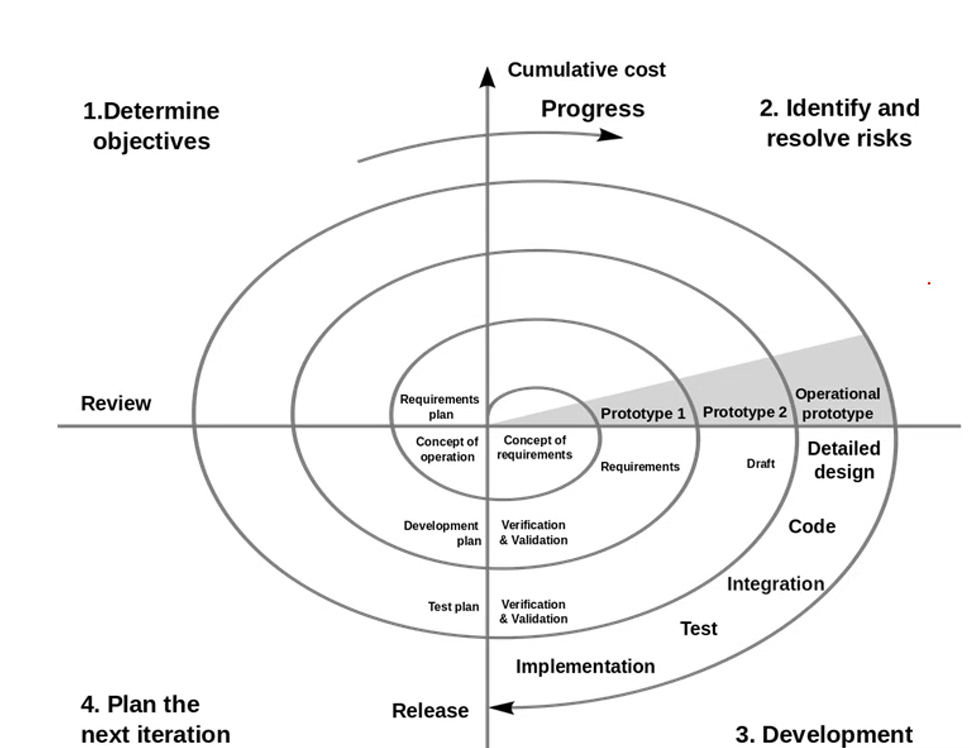
\includegraphics[scale=0.5]{p1.png}
    \caption{Spiral Model}
    \label{fig:my_label}
\end{figure}

\subsection{V Model}
\begin{itemize}
    \item The test planning and the development activity is done at the same time
    
    \item The development and testing activities form the 2 lines of the V, hence the shape and the name of the model. 
    
    \item Test planning is done early, but tests are executed only after implementation
    
    \item Apart from the shape, V also stands for \textbf{Verification} and \textbf{Validation}. 
    
    \item In a V model, every activity is sequential (one phase only starts after the previous one finishes)
\end{itemize}
\begin{figure}
    \centering
    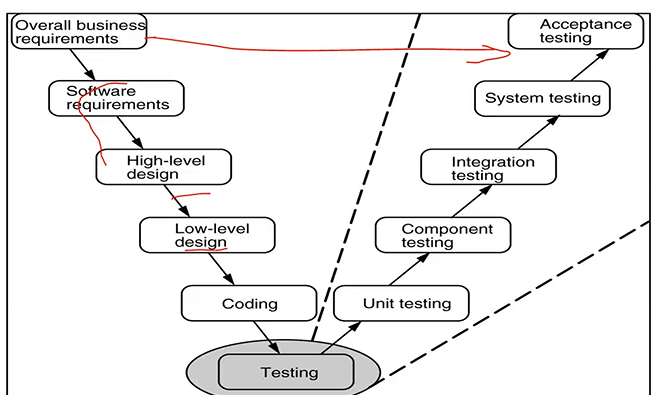
\includegraphics[scale=0.5]{p2.png}
    \caption{V Model}
    \label{fig:my_label_1}
\end{figure}

\subsection{Modified V Model}
\begin{itemize}
    \item Modified V model recognizes that different parts of a product are in different stages of evolution
    
    \item Each part entires the appropriate testing phase when the appropriate criteria are met
\end{itemize}

\section{Software Test Life Cycle}
\begin{itemize}
    \item A sequence of specific ccations performed during the testing process to ensure that softwre quality objectives are met
    
    \item Includes both verification and validation
    
    \item The phases of a normal STLC are:
    \begin{itemize}
        \item Contract Signing
        
        \item Requirement Analysis
        
        \item Test planning
        
        \item Test development
        
        \item Test environment setup
        
        \item Test execution
        
        \item Retest defects
        
        \item Closure
    \end{itemize}
\end{itemize}

\subsection{STLC Phases}
\subsubsection{Requirement Analysis}
\begin{itemize}
    \item \textbf{Entry Criteria}: SRS and architecture design available, test acceptance criteria defined
    
    \item \textbf{Activity}:
    \begin{enumerate}
        \item Identify and prioritize tests to perform
        
        \item Prepare an RTM
        
        \item Identify the test environment and perform automation feasibility analysis
    \end{enumerate}
    
    \item \textbf{Exit Criteria}: Signed off RTM and authorized automation feasibility report
    
    \item \textbf{Deliverables}: RTM, automation feasiblity report
\end{itemize}

\subsubsection{Test Planning}
\begin{itemize}
    \item \textbf{Entry Criteria}: SRS, RTM, automation feasibility report
    
    \item \textbf{Activity}:
    \begin{enumerate}
        \item Prepare test plan/strategy document
        
        \item Estimate test effort
        
        \item Resource planning
        
        \item Training requirements
    \end{enumerate}
    
    \item \textbf{Exit Criteria}: Approved test plan document, signed off effort estimate 
    
    \item \textbf{Deliverables}: Test plan document, effort estimate document
\end{itemize}

\subsubsection{Test Case Development}
\begin{itemize}
    \item \textbf{Entry Criteria}:SRS, RTM, test plan, automation analysis report
    
    \item \textbf{Activity}: 
    \begin{enumerate}
        \item Create test cases
        
        \item Automation scripts if applicable
        
        \item Review and baseline test cases/scripts
        
        \item Create test dataset
    \end{enumerate}
    
    \item \textbf{Exit Criteria}: Reviewed and signed test cases/scripts, test dataset
    
    \item \textbf{Deliverables}: Test cases, scripts, test dataset
\end{itemize}

\subsubsection{Test Environment Setup}
\begin{itemize}
    \item \textbf{Entry Criteria}: System design and architecture, environment setup plan
    
    \item \textbf{Activity}:
    \begin{enumerate}
        \item Understand the required setup
        
        \item Prepare hardware \& software requirements and envt. checklist
        
        \item Perform smoke test on build and accept based on smoke test result
    \end{enumerate}
    
    \item \textbf{Exit Criteria}: Working test envt as per plan, complete test data setup and successful smoke test
    
    \item \textbf{Deliverables}: Ready test envt and test dataset, smoke test result
\end{itemize}

\subsubsection{Test Execution}
\begin{itemize}
    \item \textbf{Entry Criteria}: Baselined RTM, test plan, test scripts/cases/envt/data, unit/integration test report
    
    \item \textbf{Activity}:
    \begin{enumerate}
        \item Run tests, document results and log defects
        
        \item Update test assets
        
        \item Map defects to test cases in RTM
        
        \item Perform regression test
    \end{enumerate}
    
    \item \textbf{Exit Criteria}: All planned tests are executed, defects logged and tracked
    
    \item \textbf{Deliverables}: Filled RTM with exec status, updated test cases and results, bug reports
\end{itemize}

\subsubsection{Test Cycle Closure}
\begin{itemize}
    \item \textbf{Entry Criteria}: Completed testing with results, defect logs available
    
    \item \textbf{Activity}: 
    \begin{enumerate}
        \item Evaluate completion critera (time, cost, coverage, biz objectives)
        
        \item Test metric calcuation
        
        \item Document learnings from project
        
        \item Prepare closure report (report of quality of work product to customer)
        
        \item Test result analysis to find distr. of bugs by type and severity
    \end{enumerate}
    
    \item \textbf{Exit Criteria}: Signed off test closure report
    
    \item \textbf{Deliverables}: Test closure report, test metrics
\end{itemize}

\section{Classification of Testing Types}
\begin{itemize}
    \item\textbf{Based on method}:
    \begin{enumerate}
        \item White-box testing
        
        \item Black-box testing
    \end{enumerate}
    
    \item \textbf{Based on requirement type}:
    \begin{enumerate}
        \item Functional testing: can be black or white box
        
        \item Non-functional testing: load/stress test, usability test, l10n testing
    \end{enumerate}
    
    \item \textbf{Based on life-cycle phase}: Focus changes from unit to sub-system to entire system
    \begin{enumerate}
        \item Unit testing: uses white-box testing
        \item Integration testing: Using white/black box tests
        \item System testing: uses black-box
    \end{enumerate}
    
    \item \textbf{Based on need}:
    \begin{enumerate}
        \item Regression testing: ensure that changes have not impacted existing behaviour
        
        \item $\alpha$ testing (limited user base, dev site) and $\beta$ testing (larger user base, cust. site)
        \item Acceptance testing
    \end{enumerate}
\end{itemize}
\end{document}
